% !TEX root = ../../../main.tex
% 来源：中学数学实验教材·第二册（几何）
% 章节：轨迹与作图 / 作图
% 原始文件：5.tex，行 668-681
% 类型：tikz
% ---
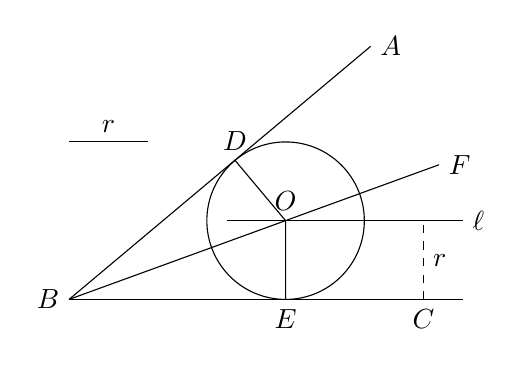
\begin{tikzpicture}[>=latex, scale=1]
\foreach \x in {0,20,40}
{
    \draw(0,0)--(\x:5);
}
\draw(2,1)--(5,1)node[right]{$\ell$};
\draw[dashed](4.5,0)node[below]{$C$}--node[right]{$r$}(4.5,1);
\draw(2.75,1) circle(1);
\draw(2.75,0)node[below]{$E$}--(2.75,1)node[above]{$O$}--(40:2.75)node[above]{$D$};
\node at (0,0) [left]{$B$};
\node at (20:5) [right]{$F$};
\node at (40:5) [right]{$A$};
\draw(0,2)--node[above]{$r$}(1,2);
    \end{tikzpicture}
